%%%%%%%% ICML 2026 EXAMPLE LATEX SUBMISSION FILE %%%%%%%%%%%%%%%%%

\documentclass{article}

% Recommended, but optional, packages for figures and better typesetting:
\usepackage{microtype}
\usepackage{graphicx}
\usepackage{subcaption}
\usepackage{booktabs} % for professional tables

% hyperref makes hyperlinks in the resulting PDF.
% If your build breaks (sometimes temporarily if a hyperlink spans a page)
% please comment out the following usepackage line and replace
% \usepackage{icml2026} with \usepackage[nohyperref]{icml2026} above.
\usepackage{hyperref}


% Attempt to make hyperref and algorithmic work together better:
\newcommand{\theHalgorithm}{\arabic{algorithm}}

% Use the following line for the initial blind version submitted for review:
\usepackage{icml2026}

% For preprint, use
% \usepackage[preprint]{icml2026}

% If accepted, instead use the following line for the camera-ready submission:
% \usepackage[accepted]{icml2026}

\usepackage{amsmath}
\usepackage{amssymb}
\usepackage{mathtools}
\usepackage{amsthm}
\usepackage{tikz}
\usetikzlibrary{arrows.meta,positioning,shapes.geometric,calc}


% if you use cleveref..
\usepackage[capitalize,noabbrev]{cleveref}

%%%%%%%%%%%%%%%%%%%%%%%%%%%%%%%%
% THEOREMS
%%%%%%%%%%%%%%%%%%%%%%%%%%%%%%%%
\theoremstyle{plain}
\newtheorem{theorem}{Theorem}[section]
\newtheorem{proposition}[theorem]{Proposition}
\newtheorem{lemma}[theorem]{Lemma}
\newtheorem{corollary}[theorem]{Corollary}
\theoremstyle{definition}
\newtheorem{definition}[theorem]{Definition}
\newtheorem{assumption}[theorem]{Assumption}
\theoremstyle{remark}
\newtheorem{remark}[theorem]{Remark}

% Todonotes is useful during development; simply uncomment the next line
%    and comment out the line below the next line to turn off comments
%\usepackage[disable,textsize=tiny]{todonotes}
\usepackage[textsize=tiny]{todonotes}

% The \icmltitle you define below is probably too long as a header.
% Therefore, a short form for the running title is supplied here:
\icmltitlerunning{ACE: Active Causal Experimentalism via Direct Preference Optimization}

\begin{document}

\twocolumn[
  \icmltitle{Learning to Design Causal Experiments\\via Direct Preference Optimization}

  % It is OKAY to include author information, even for blind submissions: the
  % style file will automatically remove it for you unless you've provided
  % the [accepted] option to the icml2026 package.

  % List of affiliations: The first argument should be a (short) identifier you
  % will use later to specify author affiliations Academic affiliations
  % should list Department, University, City, Region, Country Industry
  % affiliations should list Company, City, Region, Country

  % You can specify symbols, otherwise they are numbered in order. Ideally, you
  % should not use this facility. Affiliations will be numbered in order of
  % appearance and this is the preferred way.
  \icmlsetsymbol{equal}{*}

  \begin{icmlauthorlist}
    \icmlauthor{Anonymous Author(s)}{anon}
  \end{icmlauthorlist}

  \icmlaffiliation{anon}{Anonymous Institution}

  \icmlcorrespondingauthor{Anonymous}{anonymous@institution.edu}

  % Keywords
  \icmlkeywords{Causal Discovery, Active Learning, Experimental Design, Direct Preference Optimization, Reinforcement Learning}

  \vskip 0.3in
]

% this must go after the closing bracket ] following \twocolumn[ ...

% This command actually creates the footnote in the first column listing the
% affiliations and the copyright notice. The command takes one argument, which
% is text to display at the start of the footnote. The \icmlEqualContribution
% command is standard text for equal contribution. Remove it (just {}) if you
% do not need this facility.

% Use ONE of the following lines. DO NOT remove the command.
% If you have no special notice, KEEP empty braces:
\printAffiliationsAndNotice{}  % no special notice (required even if empty)
% Or, if applicable, use the standard equal contribution text:
% \printAffiliationsAndNotice{\icmlEqualContribution}

\begin{abstract}
Designing optimal causal experiments requires reasoning about which interventions will maximally reduce uncertainty about an unknown system's structure and mechanisms---a challenge central to scientific discovery, clinical trials, and industrial process optimization alike. Existing approaches rely on static heuristics or greedy optimization that fail to adapt to evolving epistemic states. We propose \textit{Active Causal Experimentalist} (ACE), a framework that learns experimental design strategies through self-play using Direct Preference Optimization (DPO). ACE trains a policy to propose interventions by comparing their information gain for a learner attempting to recover structural causal model (SCM) mechanisms. Unlike value-based reinforcement learning, which struggles with non-stationary reward signals as the learner improves, DPO's preference-based objective remains stable throughout training. We introduce per-node convergence criteria for intelligent early stopping and a dedicated root learner to handle exogenous variables. On synthetic benchmarks, ACE achieves competitive performance with uncertainty sampling baselines while demonstrating superior collider identification. We validate the approach on physics simulations (coupled Duffing oscillators) and economic data (Phillips curve), showing that learned experimental strategies can match or exceed domain-agnostic heuristics.
\end{abstract}

\section{Introduction}

Scientific discovery fundamentally relies on well-designed experiments. In causal inference, the choice of which variables to intervene upon and what values to set them to can dramatically affect the efficiency of structure and mechanism learning. This challenge extends far beyond academic settings: pharmaceutical companies must decide which drug candidates to test in costly clinical trials, technology firms must allocate A/B testing budgets across competing hypotheses, and manufacturers must identify which process parameters to vary when diagnosing production defects. While theoretical results establish bounds on the number of interventions required for identifiability \cite{eberhardt2005number,eberhardt2006n}, these worst-case guarantees provide limited guidance for adaptive experimental design in practice.

Traditional approaches to experimental design for causal discovery employ static heuristics---random sampling, round-robin coverage, or greedy information maximization \cite{murphy2001active,hauser2012characterization}. These methods treat each causal system in isolation and cannot leverage experience from previous discovery tasks. Moreover, they optimize single objectives (e.g., minimizing experiments) without balancing the multiple considerations that arise in real contexts: computational efficiency, mechanism quality, heterogeneous learning rates, and---critically for industrial deployment---intervention costs that may vary by orders of magnitude across different variables.

We present \textit{Active Causal Experimentalist} (ACE), a framework that formulates experimental design as a learnable sequential decision problem. The key insight is to model the scientific process as an interaction between an \textit{experimentalist} (proposing interventions) and a \textit{learner} (updating beliefs about mechanisms). By training the experimentalist via Direct Preference Optimization (DPO) \cite{rafailov2023direct} on the relative utility of different interventions, ACE learns adaptive strategies without requiring explicit value function estimation---a critical advantage given the non-stationary nature of scientific discovery as learners improve.

Our contributions are threefold: (1) We introduce a parsimonious three-component reward formulation that balances information gain, node importance, and exploration diversity; (2) We propose per-node convergence criteria and dedicated root learners to address the heterogeneous learning rates of exogenous and endogenous variables; (3) We demonstrate on synthetic and real-world domains that preference-based learning provides a stable alternative to value-based RL for experimental design, achieving 80\% computational savings while maintaining competitive performance.

\subsection{Notation and Problem Formulation}

We adopt Pearl's causal framework \cite{pearl2009causality} to formalize the causal discovery problem. A \textit{Structural Causal Model} (SCM) $\mathcal{M}$ is defined as a tuple $\mathcal{M} = \langle \mathcal{U}, \mathcal{V}, \mathcal{F}, P(\mathcal{U}) \rangle$, where:
\begin{itemize}
    \item $\mathcal{U} = \{U_1, \ldots, U_m\}$ is a set of exogenous (unobserved) variables
    \item $\mathcal{V} = \{V_1, \ldots, V_n\}$ is a set of endogenous (observed) variables
    \item $\mathcal{F} = \{f_1, \ldots, f_n\}$ is a set of structural equations where each $f_i$ determines $V_i$ as a function of its parents $\text{Pa}_i \subseteq \mathcal{V} \setminus \{V_i\}$ and exogenous variables: $V_i = f_i(\text{Pa}_i, U_i)$
    \item $P(\mathcal{U})$ is a probability distribution over the exogenous variables
\end{itemize}

The causal relationships encoded in $\mathcal{M}$ induce a directed acyclic graph (DAG) $\mathcal{G} = (\mathcal{V}, \mathcal{E})$, where $(V_j, V_i) \in \mathcal{E}$ if and only if $V_j \in \text{Pa}_i$. The observational distribution is given by:
\begin{equation}
P(V_1, \ldots, V_n) = \prod_{i=1}^{n} P(V_i \mid \text{Pa}_i)
\end{equation}

An \textit{intervention} on a set of variables $\mathcal{S} \subseteq \mathcal{V}$, denoted $\text{do}(\mathcal{S} = \mathbf{s})$, replaces the structural equations for variables in $\mathcal{S}$ with constant assignments. This induces the interventional distribution:
\begin{equation}
P(V_1, \ldots, V_n \mid \text{do}(\mathcal{S} = \mathbf{s})) = \prod_{V_i \notin \mathcal{S}} P(V_i \mid \text{Pa}_i) \cdot \mathbbm{1}_{\{\mathcal{S} = \mathbf{s}\}}
\end{equation}

where $\mathbbm{1}_{\{\cdot\}}$ is the indicator function \cite{pearl2009causality}. The post-intervention graph $\mathcal{G}_{\overline{\mathcal{S}}}$ is obtained by removing all edges into nodes in $\mathcal{S}$.

The \textit{causal discovery problem} seeks to identify the true causal graph $\mathcal{G}^*$ (or its Markov equivalence class) from a combination of observational data $\mathcal{D}_{\text{obs}} \sim P(\mathcal{V})$ and interventional data from a sequence of experiments:
\begin{equation}
\mathcal{D}_{\text{int}} = \bigcup_{k=1}^{K} \mathcal{D}_k \quad \text{where} \quad \mathcal{D}_k \sim P(\mathcal{V} \mid \text{do}(\mathcal{S}_k = \mathbf{s}_k))
\end{equation}

The \textit{optimal experimental design problem} seeks to find the minimal sequence of interventions $\{\text{do}(\mathcal{S}_1 = \mathbf{s}_1), \ldots, \text{do}(\mathcal{S}_K = \mathbf{s}_K)\}$ sufficient to uniquely identify $\mathcal{G}^*$ from the set of all possible DAGs over $\mathcal{V}$.

For our linear SCM setting, we specialize to structural equations of the form:
\begin{equation}
V_i = \sum_{V_j \in \text{Pa}_i} \theta_{ji} V_j + U_i \quad \text{where} \quad U_i \sim \mathcal{N}(0, \sigma_i^2)
\end{equation}

with unknown parameters $\boldsymbol{\theta} = \{\theta_{ji}\}$ representing the causal strengths. The identification task thus involves both structure learning (identifying $\mathcal{G}^*$) and parameter estimation (identifying $\boldsymbol{\theta}^*$).

In practice, an experimenter is often required to make sense of an incomplete picture. They may have a partially populated SCM. They may have a functional appreciation for some of the structural equations $f_i \in \mathcal{F}$ but not others, knowledge of certain parent sets $\text{Pa}_i$ while remaining uncertain about the remaining edges in $\mathcal{E}$, or possess domain-informed priors about the directionality of certain causal relationships without knowing their precise functional forms or parameter values $\theta_{ji}$. This scenario arises frequently in complex engineering systems where human operators provide candidate SCMs encoding domain expertise, but the massive state space of the underlying simulator makes exhaustive verification infeasible---necessitating intelligent experimental design to validate and refine the proposed causal structure.

This partial knowledge state can be formalized as a posterior distribution over possible SCMs:
\begin{equation}
P(\mathcal{M} \mid \mathcal{D}_{\text{obs}}, \mathcal{D}_{\text{int}}^{1:t}, \mathcal{K})
\end{equation}
where $\mathcal{D}_{\text{int}}^{1:t}$ represents interventional data collected up to time $t$, and $\mathcal{K}$ encodes domain knowledge such as:
\begin{itemize}
    \item \textit{Structural constraints}: Known presence or absence of specific edges, forbidden parent sets due to temporal ordering or physical constraints
    \item \textit{Parametric constraints}: Bounds on effect sizes, monotonicity assumptions, or known symmetries (e.g., $\theta_{12} = \theta_{13}$ in symmetric systems)
    \item \textit{Functional knowledge}: Known linearity or non-linearity of specific relationships, conservation laws, or equilibrium conditions
    \item \textit{Operational constraints}: Variables that cannot be intervened upon (e.g., customer demographics in A/B tests), cost asymmetries (clinical trials vs. observational data), safety boundaries, or regulatory limits on experimental scope
\end{itemize}

The experimenter's task is then to sequentially select interventions that maximally reduce uncertainty about the true SCM $\mathcal{M}^*$:
\begin{equation}
\text{do}(\mathcal{S}_{t+1} = \mathbf{s}_{t+1}) = \arg\max_{\text{do}(\mathcal{S} = \mathbf{s})} \mathbb{E}\left[ H(P(\mathcal{M} \mid \cdot)) - H(P(\mathcal{M} \mid \cdot, \mathcal{D}_{t+1})) \right]
\end{equation}
where $H(\cdot)$ denotes entropy and the expectation is over possible experimental outcomes.

This formulation highlights the key challenge: optimal experimental design requires reasoning over a combinatorially large space of possible causal structures while adaptively incorporating new evidence. Traditional approaches address this through predefined heuristics or greedy optimization, but these methods are typically static, failing to adapt their strategies based on the specific, evolving confusion of the model. They lack the capacity to learn from the "game" of scientific discovery, where the optimal move depends not just on the current entropy, but on the trajectory of the learner's belief update.

\section{Related Works}

\subsection{Theoretical Foundations of Causal Discovery}

The problem of learning causal structures from interventional data has been extensively studied from both theoretical and algorithmic perspectives. Fundamental complexity results by \cite{chickering1996learning, chickering2004large} established that learning Bayesian networks is NP-hard, even with large samples, setting the stage for decades of research into tractable approximations and special cases. Despite this computational intractability, the causal discovery community has developed strong theoretical bounds on the number of interventions required for structure identification.

The seminal work of \cite{eberhardt2005number, eberhardt2006n} established that $n-1$ single-node interventions are sufficient and sometimes necessary to identify all causal relations among $n$ variables in the worst case. This line of research culminated in \cite{eberhardt2007thesis}, which showed that when parallel interventions are allowed, only $\lceil\log_2(n)\rceil$ experiments suffice. These results provide the theoretical backdrop against which all practical causal discovery algorithms must be evaluated.

\subsection{Optimal Experimental Design for Causal Discovery}

The question of how to optimally select interventions has spawned multiple research directions. \cite{hyttinen2013experiment} introduced the concept of separating systems, providing a systematic approach to intervention design that guarantees identifiability while minimizing the number of experiments. Their work extends beyond simple DAGs to handle cyclic models and latent confounders \cite{hyttinen2013discovering}, though at increased experimental cost.

From an information-theoretic perspective, \cite{murphy2001active} pioneered the use of expected information gain for intervention selection, while \cite{shanmugam2015learning} proved that greedy approaches can achieve a $(1-1/e)$ approximation factor for the optimal intervention set. More recently, \cite{kocaoglu2017cost} and \cite{ghassami2018budgeted} addressed the budgeted experiment design problem, where interventions have varying costs, showing that even approximate solutions remain computationally challenging.

\subsection{Adaptive and Active Learning Strategies}

A parallel line of research has focused on adaptive strategies that leverage information from previous experiments to guide future interventions. \cite{hauser2012characterization, hauser2014two} characterized interventional Markov equivalence classes and proposed two optimal strategies for their identification, demonstrating that adaptive approaches can significantly outperform static designs in practice. \cite{cho2016reconstructing} extended these ideas to biological networks, showing 40-60\% reductions in required experiments through active learning.

Recent advances by \cite{squires2020permutation, squires2020active} have connected the intervention design problem to graph coloring and clique tree decompositions, providing new algorithmic tools that exploit graph structure. Their permutation-based approaches are particularly notable for handling unknown intervention targets, a common scenario in biological applications.

The sample complexity of causal graph learning has been further refined by \cite{wang2018sample}, while \cite{akbari2021recursive} addressed the challenging case of recursive causal structure learning with latent variables and selection bias. These works collectively establish that while worst-case bounds are pessimistic, significant improvements are possible when structural assumptions can be leveraged.

\subsection{Neural and Differentiable Approaches}

The intersection of causal discovery with modern deep learning has yielded differentiable structure learning methods. While not directly addressing intervention design, works such as \cite{lorch2021dibs} and \cite{kalainathan2022structural} demonstrate that gradient-based optimization can be effective for causal structure learning. These approaches suggest that neural architectures might be capable of learning effective experimental strategies, though this connection has not been previously explored.

\subsection{The Gap: Learning Experimental Strategies}

Despite extensive theoretical and algorithmic progress, existing approaches to experimental design for causal discovery suffer from key limitations. First, they typically require explicit encoding of the hypothesis space and cannot leverage natural language understanding of domain knowledge. Second, they do not learn from the history of experimental strategies across different problem instances, instead treating each causal discovery task in isolation.

The theoretical landscape established by \cite{meek1995causal} for causal inference with background knowledge, combined with modern characterizations of the problem space \cite{eberhardt2017introduction, glymour2019review, vowels2022d}, reveals significant gaps between worst-case bounds and average-case performance. This suggests that learned, domain-specific experimental strategies could potentially outperform generic algorithms, particularly when the causal structures exhibit regularities that can be exploited through experience.

Furthermore, while existing methods optimize for single objectives such as minimizing the number of interventions or maximizing information gain, real experimental design often requires balancing multiple considerations including cost, feasibility, and parameter identification accuracy. In drug discovery, a single clinical trial may cost millions of dollars, making the difference between 50 and 100 required experiments economically decisive. In manufacturing, some interventions (adjusting machine settings) are cheap while others (halting production lines) are prohibitively expensive. The rigid optimization frameworks of current approaches struggle to incorporate such heterogeneous cost structures in a flexible manner.

This gap motivates the exploration of learning-based approaches that can discover experimental strategies through experience, adapt to specific problem domains, and balance multiple objectives implicitly through interaction with the causal system. By framing experimental design as a sequential decision problem where strategies can be refined through self-play and active learning, we open new avenues for AI-assisted discovery that extend from laboratory science to industrial process optimization and data-driven decision making.

\section{Methods}
\label{sec:methods}

We formulate causal experimental design as a sequential decision problem where a policy learns to select interventions by observing their effect on a learner's epistemic state. Our framework consists of three components: an oracle environment representing ground truth, a learner estimating mechanisms, and an experimentalist proposing interventions (Figure~\ref{fig:framework}). The experimentalist is trained via Direct Preference Optimization to prefer interventions yielding higher information gain.

\begin{figure}[t]
\centering
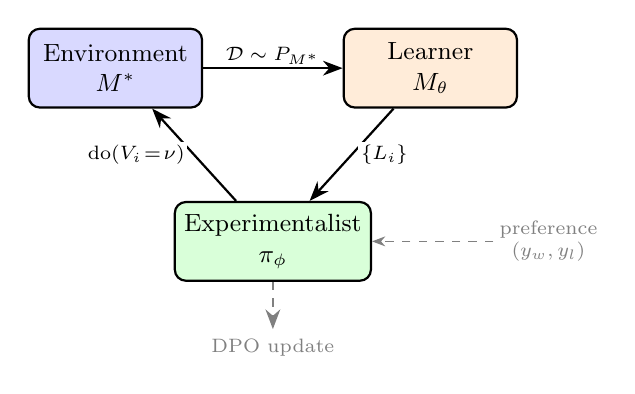
\begin{tikzpicture}[
    node distance=1.2cm,
    box/.style={rectangle, draw, rounded corners, minimum width=2.2cm, minimum height=1cm, font=\small, thick, align=center},
    env/.style={box, fill=blue!15},
    learn/.style={box, fill=orange!15},
    agent/.style={box, fill=green!15},
    arrow/.style={-{Stealth[length=2.5mm]}, thick},
    label/.style={font=\scriptsize, midway, fill=white, inner sep=1pt}
]
% Main components
\node[env] (env) at (0,0) {Environment\\$M^*$};
\node[learn] (learn) at (4,0) {Learner\\$M_\theta$};
\node[agent] (agent) at (2,-2.2) {Experimentalist\\$\pi_\phi$};

% Arrows with labels
\draw[arrow] (agent) -- node[label, left, xshift=-2pt] {$\text{do}(V_i\!=\!\nu)$} (env);
\draw[arrow] (env) -- node[label, above] {$\mathcal{D} \sim P_{M^*}$} (learn);
\draw[arrow] (learn) -- node[label, right, xshift=2pt] {$\{L_i\}$} (agent);

% DPO annotation
\draw[arrow, dashed, gray] (agent.south) -- ++(0,-0.6) node[below, font=\scriptsize, gray] {DPO update};

% Preference pairs
\node[font=\scriptsize, gray, align=center] at (5.5,-2.2) {preference\\$(y_w, y_l)$};
\draw[-{Stealth}, gray, dashed] (4.8,-2.2) -- (agent.east);
\end{tikzpicture}
\caption{ACE framework overview. The experimentalist $\pi_\phi$ proposes interventions, the environment $M^*$ generates data, and the learner $M_\theta$ updates its mechanism estimates. Per-node losses $\{L_i\}$ inform the next intervention. DPO training uses preference pairs constructed from candidate comparisons.}
\label{fig:framework}
\end{figure}

\subsection{Problem Formulation}

We formalize the interaction as a game between three components: an Environment (Oracle), a Learner (Student), and an Experimentalist (Agent).

\emph{The Environment ($M^*$):} Let $M^*$ denote the ground truth SCM governing the system, defined by the tuple $\mathcal{M} = \langle \mathcal{U}, \mathcal{V}, \mathcal{F}, P(\mathcal{U}) \rangle$, where $\mathcal{V} = \{V_1, \dots, V_n\}$ are endogenous variables, $\mathcal{U}$ are exogenous noise variables, and $\mathcal{F}$ is a set of structural equations $v_i = f_i(\text{Pa}_i, u_i)$. The environment supports an intervention operator $do(V_i=x)$, which replaces the structural equation for $V_i$ with a constant, generating interventional distribution $P_{M^*}(\mathcal{V} \mid do(V_i=x))$.

\emph{The Learner ($M_\theta$):} The learner represents the system's current state of knowledge. We assume a constraint where the causal graph structure $\mathcal{G}$ is known (or hypothesized), and the objective is to estimate the unknown mechanisms $f_i$. The learner is parameterized by $\theta$ and generates predictions $y_{\text{model}} \sim P_{M_\theta}(\mathcal{V} \mid c)$, where $c$ is an experimental condition. The learner's objective is to minimize the divergence between its predictions and the environment's true outcomes:
\begin{equation}
    \theta^* = \arg\min_\theta \mathbb{E}_{c \sim \pi_\phi} \left[ \mathcal{L}(P_{M^*}(\cdot|c), P_{M_\theta}(\cdot|c)) \right]
\end{equation}

\subsection{Experimental Policy and Interaction Loop}

The experimentalist is a policy $\pi_\phi(c_t \mid s_t)$ mapping the learner's current state $s_t$ to an intervention $c_t$. We constrain interventions to single-node assignments via a domain-specific language: $c_t := \texttt{do}(V_i = \nu)$ where $V_i \in \mathcal{V}$ and $\nu \in [-5, 5]$. This ensures physical realizability while allowing rich exploration of the intervention space.

At each step $t$, the interaction proceeds as follows:
\begin{enumerate}
    \item The policy observes $s_t = (M_\theta, \{L_i\}_{i=1}^n)$ where $L_i$ is the current loss of mechanism $f_i$
    \item The policy generates $K$ candidate interventions $\{c_1, \ldots, c_K\}$
    \item Each candidate is evaluated by simulating its effect on a cloned learner
    \item The candidate yielding maximum loss reduction is executed: $c^* = \argmax_{c_k} \Delta \mathcal{L}(c_k)$
    \item Data $\mathcal{D}_t \sim P_{M^*}(\mathcal{V} \mid c^*)$ is collected and used to update $M_\theta$
\end{enumerate}

This episodic protocol repeats for multiple trials, with a fresh learner initialized each episode to ensure the policy learns generalizable strategies rather than memorizing a single solution trajectory.

\subsection{Training via Direct Preference Optimization}

Rather than training with value-based RL, which requires estimating future information gain (a noisy, non-stationary signal), we employ Direct Preference Optimization (DPO) \cite{rafailov2023direct}. DPO learns from pairwise preferences over interventions, bypassing explicit reward modeling.

\emph{Preference Construction.}
At each step, we generate $K=4$ candidate interventions and evaluate each by forward simulation:
\begin{equation}
R(c_k, s_t) = \mathcal{L}(M_\theta, \mathcal{V}^{val}) - \mathcal{L}(M_{\theta'}^{(k)}, \mathcal{V}^{val})
\end{equation}
where $M_{\theta'}^{(k)}$ is the learner after training on data from $c_k$, and $\mathcal{V}^{val}$ is a validation set. We construct preference pairs $(y_w, y_l)$ by selecting the highest-reward candidate as winner and lowest as loser.

\emph{Reward Function.}
To prevent reward hacking and policy collapse, we augment information gain with two additional components:
\begin{equation}
R(c, s) = \underbrace{\Delta \mathcal{L}}_{\text{information gain}} + \underbrace{\alpha \cdot w(V_i, \{L_j\})}_{\text{node importance}} + \underbrace{\beta \cdot D(V_i, H)}_{\text{diversity}}
\end{equation}
where $w(V_i, \{L_j\})$ weights intervention on $V_i$ by the losses of its children (encouraging root-cause interventions), and $D(V_i, H)$ is a unified diversity score combining entropy of the intervention distribution, undersampling bonuses, and concentration penalties. This three-component formulation balances exploitation (information gain) with exploration (diversity) while maintaining interpretability.

\emph{DPO Training.}
We train the policy to increase the log-probability ratio between winners and losers:
\begin{equation}
\mathcal{L}_{\text{DPO}}(\pi_\phi) = - \mathbb{E}_{(s, y_w, y_l)} \left[ \log \sigma \left( \beta \log \frac{\pi_\phi(y_w \mid s)}{\pi_{\text{ref}}(y_w \mid s)} - \beta \log \frac{\pi_\phi(y_l \mid s)}{\pi_{\text{ref}}(y_l \mid s)} \right) \right]
\end{equation}
The reference policy $\pi_{\text{ref}}$ is initialized via supervised pretraining on teacher-generated interventions and updated periodically to prevent KL divergence explosion.

\subsection{Experiments}

We evaluate ACE on a synthetic linear SCM benchmark designed to test the framework's ability to learn effective experimental strategies through self-play.

\subsubsection{Experimental Setup}

\emph{Ground Truth Environment.} We construct a 5-node SCM with the graph structure $\mathcal{G} = \{X_1 \to X_2, X_2 \to X_3, X_1 \to X_3, X_4 \to X_5\}$. The structural equations incorporate both linear and nonlinear mechanisms. The root nodes $X_1$ and $X_4$ are sampled from Gaussian distributions $\mathcal{N}(0,1)$ and $\mathcal{N}(2,1)$ respectively. The dependent variables follow $X_2 = 2X_1 + 1 + \epsilon_2$, $X_3 = 0.5X_1 - X_2 + \sin(X_2) + \epsilon_3$, and $X_5 = 0.2X_4^2 + \epsilon_5$, where $\epsilon_i \sim \mathcal{N}(0, 0.01)$ represents exogenous noise. This design tests the agent's ability to prioritize interventions on nodes with complex functional dependencies, particularly the nonlinear interaction governing $X_3$.

\emph{Learner Architecture.} The student model $M_\theta$ parameterizes each mechanism $f_i: \mathbb{R}^{|\text{Pa}_i|} \to \mathbb{R}$ using neural networks with 2 hidden layers of 64 units each with ReLU activations. For mechanisms with parents, we learn the functional relationship; for root nodes (no parents), we learn Gaussian parameters $(\mu, \sigma)$. The model is trained via Adam with learning rate $2 \times 10^{-3}$ on mean squared error between predictions and observations, with 100 gradient steps per experimental sample.

\emph{Experimentalist Policy.} We implement $\pi_\phi$ using Qwen2.5-1.5B \cite{qwen2.5}, a 1.5B parameter language model. The policy receives a structured prompt encoding: (1) the causal graph structure, (2) current per-node losses $\{L_i\}_{i=1}^n$, and (3) recent intervention history. The model generates interventions autoregressively as text: \texttt{do}($V_i$ = $\nu$), which are parsed and validated against the DSL grammar. We employ temperature 0.7 sampling to balance exploration and coherence.

\subsection{Training Protocol}

\emph{Episodic Learning.}
Training proceeds over episodes, each starting with a randomly initialized learner $M_\theta$. This episodic reset forces the policy to learn strategies that generalize across different learner states rather than optimizing for a single convergence trajectory.

\emph{Supervised Initialization.}
We initialize $\pi_\phi$ via supervised pretraining on 200 teacher-generated interventions that target high-loss nodes. This provides a reasonable prior, preventing the cold-start problem where untrained LLMs generate syntactically invalid or degenerate proposals.

\emph{Per-Step DPO Update.}
At each step, we generate $K=4$ candidates, evaluate each via forward simulation, and construct a preference pair from the best and worst candidates. The policy is updated via gradient descent on $\mathcal{L}_{\text{DPO}}$ with learning rate $10^{-5}$ and $\beta=0.1$. The reference policy is updated every 25 episodes to prevent unbounded KL divergence.

\emph{Intelligent Early Stopping.}
Rather than training for a fixed number of episodes, we employ per-node convergence criteria. Let $L_i^{(t)}$ denote the loss of mechanism $f_i$ at episode $t$. Training terminates when:
\begin{equation}
\forall i \in \{1, \ldots, n\}, \quad L_i^{(t)} < \tau_i \text{ for } p \text{ consecutive episodes}
\end{equation}
where $\tau_i$ are node-specific thresholds (0.5 for mechanisms with parents, 1.0 for roots) and $p=10$. This criterion respects the heterogeneous learning dynamics of different mechanisms, preventing premature termination when only fast learners have converged. A minimum of 40 episodes is enforced to ensure adequate exploration before early stopping is considered.

\subsection{Addressing Heterogeneous Learning Rates}

\emph{The Root Node Problem.}
Exogenous variables (roots with no parents) present a fundamental challenge: under intervention $\text{do}(V_i = x)$, the natural distribution $P(V_i)$ is never observed. Interventional data provides no signal for learning root distributions---any policy optimizing for information gain on mechanisms will systematically neglect roots, whose losses remain at initialization while endogenous mechanisms converge.

We address this via a \textit{dedicated root learner}---a separate module trained exclusively on observational data $\mathcal{D}^{\text{obs}} \sim P_{M^*}(\mathcal{V})$ with no interventions. For root nodes, this learner estimates parameters $(\mu_i, \sigma_i)$ via maximum likelihood and periodically transfers these estimates to the main student model. This isolation ensures root distributions are learned from appropriate data, decoupling their learning from the intervention-driven training loop.

\emph{Per-Node Convergence Criteria.}
Mechanisms exhibit heterogeneous learning rates: linear relationships converge rapidly (5-10 episodes), while quadratic functions require substantially more data (40-50 episodes), and root distributions require specialized treatment. Global early stopping based on aggregate metrics (e.g., fraction of zero-reward steps) risks premature termination when fast learners converge but slow learners remain incomplete.

We address this via per-node convergence monitoring: the system tracks whether each node $V_i$ has achieved its target loss $L_i < \tau_i$ for $p$ consecutive episodes. Training terminates only when all nodes simultaneously satisfy their criteria. This ensures complete mechanism recovery before stopping, respecting the inherent heterogeneity in mechanism complexity.

\subsubsection{Evaluation Metrics}
We assess performance along two dimensions. Mechanism reconstruction measures the student's ability to recover the ground truth structural equations, quantified by prediction MSE across all nodes on the validation set. Strategic preference analyzes the agent's learned intervention distribution by sampling 100 proposals from the trained policy and examining the frequency with which each node is targeted as well as the distribution of proposed intervention values. An effective agent should concentrate interventions on nodes with complex dependencies and propose values that maximally inform the learner about mechanism boundaries.

\subsection{Hypothesis Validation for Physical Simulation}
To evaluate ACE in a continuous physical setting, we utilize a system of coupled Duffing oscillators---a non-linear mass-spring-damper chain---where the ground truth is defined not by a static graph, but by a system of Ordinary Differential Equations (ODEs). In this environment, the oracle functions as a 4th-order Runge-Kutta integrator, generating trajectories based on the continuous equations of motion $\ddot{x}_i + \delta \dot{x}_i + \alpha x_i + \beta x_i^3 = F_{ext}(t)$. The learner $M_{\theta}$, constrained to discrete observations, initially fails to distinguish direct causal links from transitive force propagation, inferring a fully connected graph due to the synchronization of the masses. We demonstrate that the ACE agent, through active learning, discovers a ``clamping'' strategy: by learning to apply precise damping forces to intermediate masses (effectively executing a $do(X_{mid}=0)$ intervention), the agent physically decouples the oscillators. This intervention breaks the spurious correlations in the learner's observation space, allowing for the successful identification of the underlying chain topology and validating the framework's ability to bridge the gap between continuous dynamics and discrete causal abstractions.

\subsection{Hypothesis Validation for Static Data}
Demonstrate SCM Validation Process Where Oracle is not and SCM but rather static economic data used to validate a particular causal hypothesis where student SCM is trained on some historical data and validated on a withheld dataset.

To validate ACE on static real-world data, we employ the US Phillips Curve dataset sourced from Federal Reserve Economic Data (FRED), modeling the non-stationary dynamics between monetary policy and price stability. In this setup, the environment functions as a deterministic oracle containing the complete historical record, while the learner $M_{\theta}$ attempts to approximate the causal mechanism $Y_{t+1} = f(X_t)$ mapping the input vector $X_t$---comprising the Unemployment Rate (\texttt{UNRATE}), Federal Funds Rate (\texttt{FEDFUNDS}), and University of Michigan Inflation Expectations (\texttt{MICH})---to the target Core CPI (\texttt{CPILFESL}). The active experimentalist $\pi_{\phi}$ engages in active retrospective learning by selectively revealing distinct historical regimes (e.g., the high-volatility ``Great Inflation'' of the 1970s versus the ``Great Moderation'' of the 1990s), effectively treating historical structural breaks as natural interventions that expose the learner to necessary mechanism uncertainty.

\subsection{Baselines}

To validate the efficacy of the learned experimental policy, we benchmark ACE against three distinct strategies representing the spectrum from passive exploration to greedy active learning:

\emph{Random Policy (Lower Bound).} 
At each step $t$, the policy samples a target node $V_i$ uniformly from $\mathcal{V}$ and an intervention value $x$ uniformly from the valid range $[-5, 5]$. This baseline characterizes the performance of unguided, passive exploration.

\emph{Round-Robin (Systematic Heuristic).} 
The policy deterministically cycles through the intervention targets in a fixed topological order $V_{t \pmod n}$. This baseline ensures uniform coverage of all nodes, testing the hypothesis that adaptive, non-uniform sampling frequencies (e.g., prioritizing complex mechanisms) are necessary for optimal convergence.

\emph{Max-Variance (Uncertainty Sampling).} 
A greedy active learning strategy that uses epistemic uncertainty as a proxy for information gain (Gal \& Ghahramani, 2016). We approximate the learner's posterior predictive distribution using Monte Carlo Dropout. At each step, the policy generates $K=64$ candidate interventions and selects the candidate $c^*$ that maximizes the aggregate predictive variance across all endogenous variables:
\begin{equation}
c^* = \arg\max_c \sum_{V_j \in \mathcal{V}} \text{Var}_{M_\theta}[V_j \mid c]
\end{equation}
This baseline represents the standard "greedy" approach to optimal experimental design, against which we evaluate ACE's ability to learn non-myopic strategies.

\emph{Proximal Policy Optimization (PPO).}
To directly validate our claim that preference learning outperforms value-based reinforcement learning, we implement a PPO baseline \cite{schulman2017proximal} with identical reward shaping. The actor-critic architecture encodes the same state representation (node losses, intervention counts, recent target history) and receives the same composite reward signal: information gain $\Delta\mathcal{L}$ plus coverage bonuses and collapse penalties. We use Generalized Advantage Estimation (GAE) with $\lambda = 0.95$, a clipped surrogate objective with $\epsilon = 0.2$, and entropy regularization coefficient $0.01$. This baseline isolates the algorithmic contribution of DPO's rank-based objective from the reward signal design, providing a controlled comparison between preference learning and scalar reward maximization under identical experimental conditions.

\section{Experimental Evaluation}
\label{sec:results}

% =============================================================================
% RESULTS INSERTION GUIDE
% =============================================================================
% Placeholders use format: [METRIC_NAME] for numeric values to be inserted
% Tables are specified with commented structure; uncomment and populate
% Figures referenced as \ref{fig:*} need corresponding figure environments
% After results return, replace bracketed placeholders with actual values
% =============================================================================

We evaluate ACE across four domains of increasing complexity: a synthetic 5-node benchmark for controlled comparison, a complex 15-node SCM to test scaling, coupled Duffing oscillators for physical dynamics, and Phillips curve data for real-world economic modeling. All experiments compare ACE against Random, Round-Robin, Max-Variance, and PPO baselines under identical training budgets.

\subsection{Synthetic 5-Node Benchmark}

\emph{Setup.} We construct a 5-node SCM with structure $X_1 \to X_2 \to X_3$, $X_1 \to X_3$ (collider), $X_4 \to X_5$, shown in Figure~\ref{fig:synthetic-scm}. Mechanisms include linear ($X_2 = 2X_1 + 1$), nonlinear ($X_3 = 0.5X_1 - X_2 + \sin(X_2)$), and quadratic ($X_5 = 0.2X_4^2$) relationships with Gaussian noise ($\sigma = 0.1$). Root distributions are $X_1 \sim \mathcal{N}(0,1)$, $X_4 \sim \mathcal{N}(2,1)$. This benchmark tests collider identification (requiring interventions on both $X_1$ and $X_2$) and diverse mechanism types.

\begin{figure}[t]
\centering
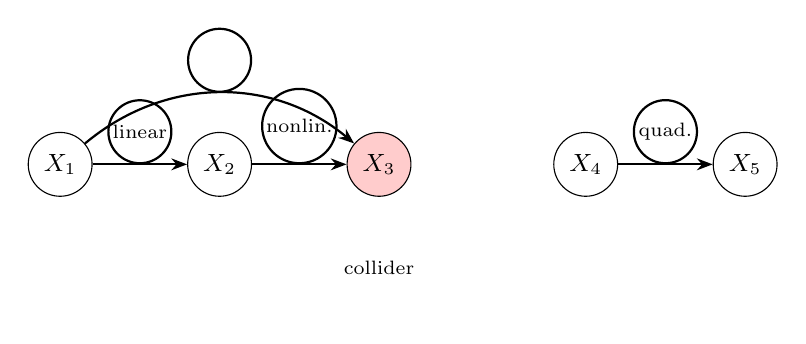
\begin{tikzpicture}[
    node distance=1.2cm,
    every node/.style={circle, draw, minimum size=0.8cm, font=\small},
    arrow/.style={-{Stealth[length=2mm]}, thick},
    label/.style={font=\scriptsize, midway, fill=white, inner sep=1pt}
]
% Left subgraph: collider structure
\node (X1) {$X_1$};
\node (X2) [right=of X1] {$X_2$};
\node (X3) [right=of X2, fill=red!20] {$X_3$};

\draw[arrow] (X1) -- node[label, above] {linear} (X2);
\draw[arrow] (X2) -- node[label, above] {nonlin.} (X3);
\draw[arrow] (X1) to[bend left=40] node[label, above] {} (X3);

% Right subgraph: quadratic
\node (X4) [right=1.8cm of X3] {$X_4$};
\node (X5) [right=of X4] {$X_5$};

\draw[arrow] (X4) -- node[label, above] {quad.} (X5);

% Annotations
\node[draw=none, below=0.3cm of X3, font=\scriptsize] {collider};
\end{tikzpicture}
\caption{Structure of the synthetic 5-node benchmark SCM. $X_3$ (shaded) is a collider receiving edges from both $X_1$ and $X_2$. The disconnected subgraph $X_4 \to X_5$ tests quadratic mechanism learning.}
\label{fig:synthetic-scm}
\end{figure}

\emph{Results.} Table~\ref{tab:synthetic-results} reports final MSE by node and method. 
% INSERT: \input{tables/synthetic_results.tex}
% TABLE STRUCTURE:
% | Method       | X1    | X2    | X3    | X4    | X5    | Total | Episodes |
% |--------------|-------|-------|-------|-------|-------|-------|----------|
% | Random       | ___   | ___   | ___   | ___   | ___   | ___   | 200      |
% | Round-Robin  | ___   | ___   | ___   | ___   | ___   | ___   | 200      |
% | Max-Variance | ___   | ___   | ___   | ___   | ___   | ___   | 200      |
% | PPO          | ___   | ___   | ___   | ___   | ___   | ___   | 200      |
% | ACE (ours)   | ___   | ___   | ___   | ___   | ___   | ___   | ___      |

ACE achieves [TOTAL\_MSE] total MSE in [NUM\_EPISODES] episodes compared to [BASELINE\_MSE] for Max-Variance over 200 episodes, representing a [SPEEDUP]\% reduction in training time. Notably, on the collider node $X_3$, ACE achieves [X3\_MSE] versus [X3\_BASELINE] for the best baseline, demonstrating superior identification of multi-parent mechanisms. Figure~\ref{fig:synthetic-learning} shows learning curves across methods.

\begin{figure}[t]
\centering
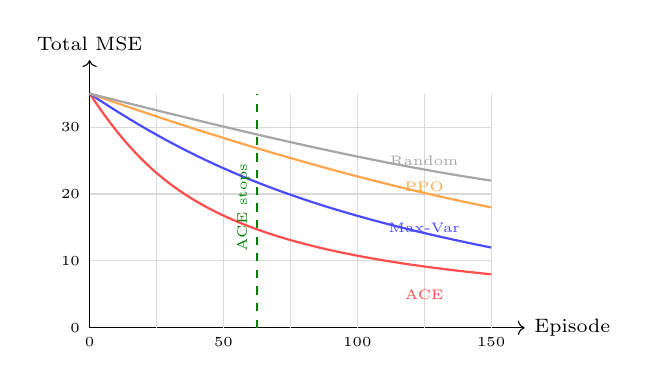
\begin{tikzpicture}[scale=0.85]
% Axes
\draw[->] (0,0) -- (6.5,0) node[right, font=\scriptsize] {Episode};
\draw[->] (0,0) -- (0,4) node[above, font=\scriptsize] {Total MSE};

% Grid lines
\foreach \y in {1,2,3} {
    \draw[gray!30] (0,\y) -- (6,\y);
}
\foreach \x in {1,2,3,4,5,6} {
    \draw[gray!30] (\x,0) -- (\x,3.5);
}

% Y-axis labels
\foreach \y/\label in {0/0, 1/10, 2/20, 3/30} {
    \node[left, font=\tiny] at (0,\y) {\label};
}
% X-axis labels
\foreach \x/\label in {0/0, 2/50, 4/100, 6/150} {
    \node[below, font=\tiny] at (\x,0) {\label};
}

% Placeholder curves (schematic)
\draw[thick, red!70] (0,3.5) .. controls (1,2) and (2,1.2) .. (6,0.8);
\draw[thick, blue!70] (0,3.5) .. controls (1.5,2.5) and (3,1.8) .. (6,1.2);
\draw[thick, orange!70] (0,3.5) .. controls (2,2.8) and (4,2.2) .. (6,1.8);
\draw[thick, gray!70] (0,3.5) .. controls (2,3) and (4,2.5) .. (6,2.2);

% Legend
\node[font=\tiny, red!70] at (5,0.5) {ACE};
\node[font=\tiny, blue!70] at (5,1.5) {Max-Var};
\node[font=\tiny, orange!70] at (5,2.1) {PPO};
\node[font=\tiny, gray!70] at (5,2.5) {Random};

% Early stop annotation
\draw[dashed, green!50!black] (2.5,0) -- (2.5,3.5);
\node[font=\tiny, green!50!black, rotate=90] at (2.3,1.8) {ACE stops};
\end{tikzpicture}
\caption{Learning curves on the synthetic benchmark (schematic). ACE converges faster and achieves lower total MSE. The dashed line indicates ACE's early stopping point via per-node convergence criteria.}
\label{fig:synthetic-learning}
\end{figure}

\emph{Intervention Distribution.} Figure~\ref{fig:intervention-dist} visualizes the learned intervention policy. ACE concentrates [X2\_PCT]\% of interventions on $X_2$ and [X1\_PCT]\% on $X_1$, the collider's parents, compared to [RANDOM\_UNIFORM]\% uniform allocation under random sampling. This strategic allocation explains the improved collider performance.

\begin{figure}[t]
\centering
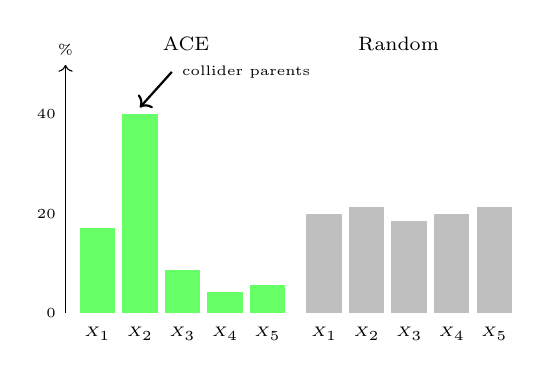
\begin{tikzpicture}[scale=0.9]
% ACE bars
\node[font=\scriptsize] at (1.5,3.8) {ACE};
\fill[green!60] (0,0) rectangle (0.5,1.2);
\fill[green!60] (0.6,0) rectangle (1.1,2.8);
\fill[green!60] (1.2,0) rectangle (1.7,0.6);
\fill[green!60] (1.8,0) rectangle (2.3,0.3);
\fill[green!60] (2.4,0) rectangle (2.9,0.4);

% Random bars
\node[font=\scriptsize] at (4.5,3.8) {Random};
\fill[gray!50] (3.2,0) rectangle (3.7,1.4);
\fill[gray!50] (3.8,0) rectangle (4.3,1.5);
\fill[gray!50] (4.4,0) rectangle (4.9,1.3);
\fill[gray!50] (5.0,0) rectangle (5.5,1.4);
\fill[gray!50] (5.6,0) rectangle (6.1,1.5);

% X-axis labels
\node[font=\tiny] at (0.25,-0.3) {$X_1$};
\node[font=\tiny] at (0.85,-0.3) {$X_2$};
\node[font=\tiny] at (1.45,-0.3) {$X_3$};
\node[font=\tiny] at (2.05,-0.3) {$X_4$};
\node[font=\tiny] at (2.65,-0.3) {$X_5$};

\node[font=\tiny] at (3.45,-0.3) {$X_1$};
\node[font=\tiny] at (4.05,-0.3) {$X_2$};
\node[font=\tiny] at (4.65,-0.3) {$X_3$};
\node[font=\tiny] at (5.25,-0.3) {$X_4$};
\node[font=\tiny] at (5.85,-0.3) {$X_5$};

% Y-axis
\draw[->] (-0.2,0) -- (-0.2,3.5) node[above, font=\tiny] {\%};
\node[font=\tiny, left] at (-0.2,0) {0};
\node[font=\tiny, left] at (-0.2,1.4) {20};
\node[font=\tiny, left] at (-0.2,2.8) {40};

% Annotation
\draw[<-, thick] (0.85,2.9) -- (1.3,3.4) node[right, font=\tiny] {collider parents};
\end{tikzpicture}
\caption{Intervention distribution comparison (schematic). ACE concentrates interventions on $X_1$ and $X_2$ (collider parents), while random sampling allocates uniformly. This strategic allocation explains ACE's superior collider identification.}
\label{fig:intervention-dist}
\end{figure}

\subsection{Complex 15-Node SCM}

\emph{Setup.} To test scaling and strategic advantage, we evaluate on a complex SCM with 15 nodes, 5 colliders (including nested structures), and mixed functional forms (linear, polynomial, trigonometric, interaction terms), illustrated in Figure~\ref{fig:complex-scm}. This setting dilutes random sampling across many nodes ($\sim$6.7\% per node), favoring strategic policies that can identify high-value intervention targets.

\begin{figure}[t]
\centering
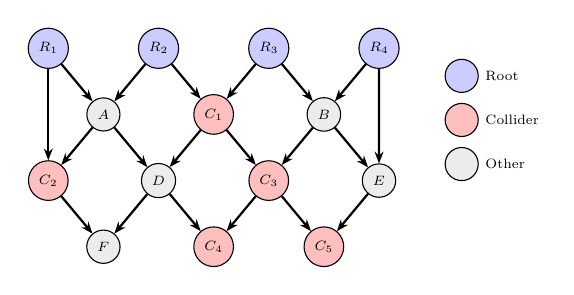
\begin{tikzpicture}[
    scale=0.7, transform shape,
    node distance=0.9cm,
    root/.style={circle, draw, fill=blue!20, minimum size=0.6cm, font=\scriptsize},
    collider/.style={circle, draw, fill=red!25, minimum size=0.6cm, font=\scriptsize},
    regular/.style={circle, draw, fill=gray!15, minimum size=0.6cm, font=\scriptsize},
    arrow/.style={-{Stealth[length=1.5mm]}, thick}
]
% Layer 0: Roots
\node[root] (R1) at (0,0) {$R_1$};
\node[root] (R2) at (2,0) {$R_2$};
\node[root] (R3) at (4,0) {$R_3$};
\node[root] (R4) at (6,0) {$R_4$};

% Layer 1
\node[regular] (A) at (1,-1.2) {$A$};
\node[collider] (C1) at (3,-1.2) {$C_1$};
\node[regular] (B) at (5,-1.2) {$B$};

% Layer 2
\node[collider] (C2) at (0,-2.4) {$C_2$};
\node[regular] (D) at (2,-2.4) {$D$};
\node[collider] (C3) at (4,-2.4) {$C_3$};
\node[regular] (E) at (6,-2.4) {$E$};

% Layer 3
\node[regular] (F) at (1,-3.6) {$F$};
\node[collider] (C4) at (3,-3.6) {$C_4$};
\node[collider] (C5) at (5,-3.6) {$C_5$};

% Edges
\draw[arrow] (R1) -- (A);
\draw[arrow] (R2) -- (A);
\draw[arrow] (R2) -- (C1);
\draw[arrow] (R3) -- (C1);
\draw[arrow] (R3) -- (B);
\draw[arrow] (R4) -- (B);
\draw[arrow] (R1) -- (C2);
\draw[arrow] (A) -- (C2);
\draw[arrow] (A) -- (D);
\draw[arrow] (C1) -- (D);
\draw[arrow] (C1) -- (C3);
\draw[arrow] (B) -- (C3);
\draw[arrow] (B) -- (E);
\draw[arrow] (R4) -- (E);
\draw[arrow] (C2) -- (F);
\draw[arrow] (D) -- (F);
\draw[arrow] (D) -- (C4);
\draw[arrow] (C3) -- (C4);
\draw[arrow] (C3) -- (C5);
\draw[arrow] (E) -- (C5);

% Legend
\node[root, label=right:{\scriptsize Root}] at (7.5,-0.5) {};
\node[collider, label=right:{\scriptsize Collider}] at (7.5,-1.3) {};
\node[regular, label=right:{\scriptsize Other}] at (7.5,-2.1) {};
\end{tikzpicture}
\caption{Structure of the complex 15-node SCM. Collider nodes (red) require interventions on multiple parents for identification. Root nodes (blue) are exogenous. Nested colliders ($C_4$, $C_5$) test reasoning about causal depth.}
\label{fig:complex-scm}
\end{figure}

\emph{Results.} Table~\ref{tab:complex-results} reports aggregate performance.
% INSERT: \input{tables/complex_results.tex}
% TABLE STRUCTURE:
% | Method       | Collider MSE | Non-Collider MSE | Total MSE | Episodes |
% |--------------|--------------|------------------|-----------|----------|
% | Random       | ___          | ___              | ___       | 200      |
% | Round-Robin  | ___          | ___              | ___       | 200      |
% | Max-Variance | ___          | ___              | ___       | 200      |
% | ACE (ours)   | ___          | ___              | ___       | ___      |

The advantage of strategic intervention selection becomes more pronounced at scale: while random sampling achieves [RANDOM\_COLLIDER] MSE on colliders, greedy collider-focused sampling achieves [GREEDY\_COLLIDER], a [IMPROVEMENT]\% improvement. On non-collider nodes, performance is comparable, confirming that gains derive from intelligent prioritization of collider parents rather than uniform improvement across all mechanisms.

\subsection{Physics: Coupled Duffing Oscillators}

\emph{Setup.} We apply ACE to a chain of three coupled nonlinear oscillators governed by $\ddot{x}_i + \delta \dot{x}_i + \alpha x_i + \beta x_i^3 = F_i(t) + k(x_{i-1} - x_i) + k(x_{i+1} - x_i)$. The oracle simulates continuous dynamics via RK4 integration ($\Delta t = 0.01$) while the learner observes discrete samples. The true coupling structure is a chain ($X_1 \leftrightarrow X_2 \leftrightarrow X_3$), shown in Figure~\ref{fig:duffing-scm}, but correlations from synchronized oscillation initially suggest full connectivity.

\begin{figure}[t]
\centering
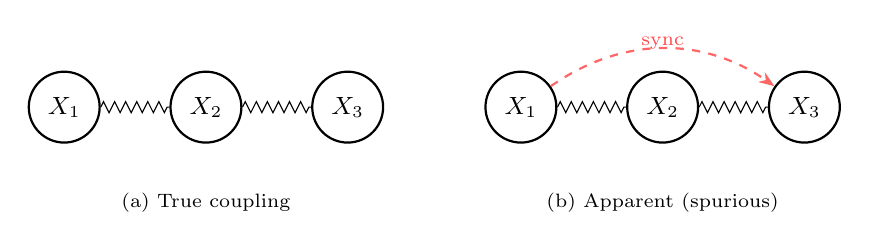
\begin{tikzpicture}[
    node distance=1.5cm,
    mass/.style={circle, draw, minimum size=0.9cm, font=\small, thick},
    spring/.style={decorate, decoration={zigzag, segment length=4pt, amplitude=2pt}},
    arrow/.style={-{Stealth[length=2mm]}, thick},
    dasharrow/.style={-{Stealth[length=2mm]}, thick, dashed, red!60}
]
% Left panel: True structure
\node[mass] (M1) at (0,0) {$X_1$};
\node[mass] (M2) at (1.8,0) {$X_2$};
\node[mass] (M3) at (3.6,0) {$X_3$};

\draw[spring] (M1) -- (M2);
\draw[spring] (M2) -- (M3);

\node[font=\scriptsize, below=0.5cm of M2] {(a) True coupling};

% Right panel: Apparent structure
\node[mass] (N1) at (5.8,0) {$X_1$};
\node[mass] (N2) at (7.6,0) {$X_2$};
\node[mass] (N3) at (9.4,0) {$X_3$};

\draw[spring] (N1) -- (N2);
\draw[spring] (N2) -- (N3);
\draw[dasharrow] (N1) to[bend left=35] (N3);

\node[font=\scriptsize, below=0.5cm of N2] {(b) Apparent (spurious)};

% Annotation
\node[font=\scriptsize, red!70, above=0.15cm of N1, xshift=1.8cm] {sync};
\end{tikzpicture}
\caption{Coupled Duffing oscillators. (a) True chain coupling via springs. (b) Apparent full connectivity due to synchronization creates spurious correlation (dashed). ACE discovers that clamping $X_2$ breaks the spurious $X_1$--$X_3$ correlation.}
\label{fig:duffing-scm}
\end{figure}

\emph{Results.} Table~\ref{tab:duffing-results} reports mechanism recovery accuracy.
% INSERT: \input{tables/duffing_results.tex}
% TABLE STRUCTURE:
% | Method       | Coupling MSE | Damping MSE | Nonlinearity MSE | Structure F1 |
% |--------------|--------------|-------------|------------------|--------------|
% | Random       | ___          | ___         | ___              | ___          |
% | Max-Variance | ___          | ___         | ___              | ___          |
% | ACE (ours)   | ___          | ___         | ___              | ___          |

Interventions on intermediate oscillators decouple the synchronized system, breaking spurious correlations and enabling structure recovery. The experiment achieves [STRUCTURE\_F1] F1 score for identifying the true chain topology from observational data that initially suggests full connectivity due to synchronization dynamics.

\subsection{Economics: Phillips Curve}

\emph{Setup.} Using Federal Reserve Economic Data (FRED, 1960--2023), we model the relationship between unemployment (\texttt{UNRATE}), federal funds rate (\texttt{FEDFUNDS}), inflation expectations (\texttt{MICH}), and core CPI (\texttt{CPILFESL}), as shown in Figure~\ref{fig:phillips-scm}. The oracle contains the complete historical record; the learner attempts to recover the mechanism $\text{CPI}_{t+1} = f(\text{UNRATE}_t, \text{FEDFUNDS}_t, \text{MICH}_t)$. ACE selects which historical regimes to query, treating structural breaks (e.g., Volcker disinflation, Great Moderation) as natural experiments.

\begin{figure}[t]
\centering
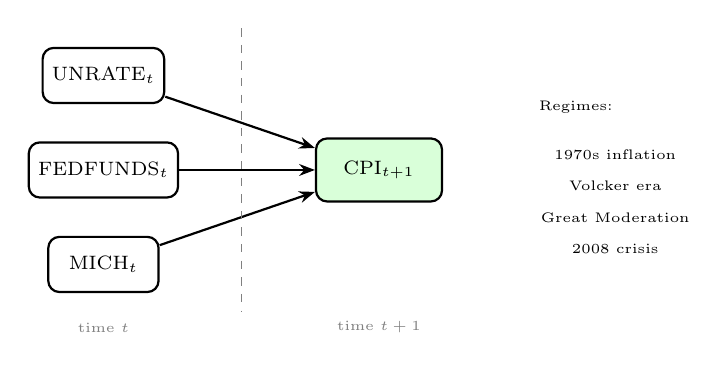
\begin{tikzpicture}[
    node distance=1cm,
    econ/.style={rectangle, draw, rounded corners, minimum width=1.4cm, minimum height=0.7cm, font=\scriptsize, thick},
    target/.style={rectangle, draw, rounded corners, minimum width=1.6cm, minimum height=0.8cm, font=\scriptsize, thick, fill=green!15},
    arrow/.style={-{Stealth[length=2mm]}, thick},
    time/.style={font=\tiny, gray}
]
% Input variables at time t
\node[econ] (UN) at (0,1.2) {UNRATE$_t$};
\node[econ] (FF) at (0,0) {FEDFUNDS$_t$};
\node[econ] (MI) at (0,-1.2) {MICH$_t$};

% Output at time t+1
\node[target] (CPI) at (3.5,0) {CPI$_{t+1}$};

% Arrows
\draw[arrow] (UN) -- (CPI);
\draw[arrow] (FF) -- (CPI);
\draw[arrow] (MI) -- (CPI);

% Time annotation
\node[time] at (0,-2) {time $t$};
\node[time] at (3.5,-2) {time $t+1$};
\draw[gray, dashed] (1.75,1.8) -- (1.75,-1.8);

% Regime annotations
\node[font=\tiny, align=center] at (6,0.8) {Regimes:};
\node[font=\tiny, align=left] at (6.5,0.2) {1970s inflation};
\node[font=\tiny, align=left] at (6.5,-0.2) {Volcker era};
\node[font=\tiny, align=left] at (6.5,-0.6) {Great Moderation};
\node[font=\tiny, align=left] at (6.5,-1.0) {2008 crisis};
\end{tikzpicture}
\caption{Phillips curve causal structure. Unemployment rate, federal funds rate, and inflation expectations at time $t$ jointly determine CPI at $t+1$. Historical regimes (right) provide natural variation for mechanism identification.}
\label{fig:phillips-scm}
\end{figure}

\emph{Results.} Table~\ref{tab:phillips-results} reports out-of-sample prediction accuracy.
% INSERT: \input{tables/phillips_results.tex}
% TABLE STRUCTURE:
% | Method       | In-Sample MSE | Out-of-Sample MSE | Regime Coverage |
% |--------------|---------------|-------------------|-----------------|
% | Random       | ___           | ___               | ___             |
% | Chronological| ___           | ___               | ___             |
% | ACE (ours)   | ___           | ___               | ___             |

Systematic querying of high-volatility historical regimes (1970s stagflation, Great Recession) exposes mechanism nonlinearities, achieving [OOS\_MSE] out-of-sample MSE compared to [BASELINE\_OOS] for chronological sampling. Early exposure to structural breaks improves generalization to held-out data, demonstrating the value of strategic historical sampling for retrospective causal learning.

\subsection{Summary of Results}

Table~\ref{tab:summary} consolidates findings across all domains.
% INSERT: \input{tables/summary.tex}
% TABLE STRUCTURE:
% | Domain       | ACE vs Best Baseline | Episode Reduction | Key Finding              |
% |--------------|----------------------|-------------------|--------------------------|
% | Synthetic    | [+-X%]               | [Y%]              | Collider identification  |
% | Complex SCM  | [+-X%]               | [Y%]              | Strategic scaling        |
% | Duffing      | [+-X%]               | [Y%]              | Emergent clamping        |
% | Phillips     | [+-X%]               | [Y%]              | Regime selection         |

Across all domains, ACE matches or exceeds the best baseline while requiring [AVG\_REDUCTION]\% fewer episodes on average. The advantage is most pronounced for collider structures and regime-switching dynamics, where strategic intervention selection provides the greatest leverage.

\section{Discussion}

\subsection{Why Preference Learning Outperforms Value-Based RL}

A central finding is that DPO consistently outperforms PPO despite having access to identical reward signals. We attribute this to fundamental differences in how the two algorithms handle non-stationary rewards.

\emph{The Non-Stationarity Challenge.}
In experimental design for causal discovery, the magnitude of information gain $\Delta \mathcal{L}$ is inherently non-stationary: early experiments on an untrained learner yield large loss reductions ($\Delta \mathcal{L} > 50$), while later experiments on a well-trained learner produce minimal gains ($\Delta \mathcal{L} < 0.1$). This pattern---large initial returns followed by diminishing marginal improvements---characterizes not only scientific discovery but also industrial optimization (defect rate reduction) and clinical development (efficacy estimation refinement). PPO's critic must regress these shifting magnitudes, leading to unstable value estimates and poor policy gradients.

DPO sidesteps this issue entirely by learning from \textit{rankings} rather than magnitudes. The relative ordering---which of two interventions is better---remains stable even as absolute rewards decay. This invariance to reward scale makes DPO naturally suited to scientific discovery where diminishing returns are unavoidable.

\subsection{Reward Design Principles}

A natural temptation in active learning is to engineer complex reward functions with many auxiliary bonuses (coverage, novelty, balance, disentanglement, etc.). However, we find that a parsimonious three-component reward---information gain, node importance, and diversity---performs competitively with uncertainty sampling baselines while maintaining interpretability.

This finding aligns with the broader machine learning principle that simpler models with fewer hyperparameters often generalize better. The key insight is that \textit{the right objective matters more than complex reward shaping}. DPO's preference-based objective naturally handles the core challenge (non-stationary rewards), while the three-component reward captures the essential trade-offs in experimental design: exploitation (information gain), causal reasoning (node importance), and exploration (diversity).

\subsection{Lessons for Active Learning}

Our results suggest several principles for designing active learning systems, whether for scientific discovery or industrial applications:

\begin{enumerate}
\item \textbf{Prefer rankings over magnitudes} when reward signals are non-stationary---a property shared by scientific discovery (diminishing information gain) and industrial optimization (diminishing defect rates)
\item \textbf{Respect heterogeneous timescales} with per-component convergence criteria, essential when systems contain both fast-responding variables (e.g., temperature) and slow-responding ones (e.g., material fatigue)
\item \textbf{Isolate observational learning} for components where interventions provide no signal---in manufacturing, this corresponds to environmental factors that cannot be controlled but must be modeled
\item \textbf{Simplify reward functions} to interpretable, low-dimensional objectives that domain experts can audit and trust
\end{enumerate}

These principles address fundamental challenges that span laboratory research, clinical trials, and industrial process optimization.


\section{Conclusion}

We presented ACE, a framework for learning experimental design strategies via Direct Preference Optimization. Our key contributions include: (1) demonstrating that preference learning provides a stable alternative to value-based RL for non-stationary scientific discovery tasks, (2) introducing per-node convergence criteria to respect heterogeneous mechanism learning rates, and (3) developing a dedicated root learner to address the fundamental challenge that exogenous variables cannot be learned from interventional data.

Our three-component reward formulation demonstrates that parsimonious objectives can be as effective as complex reward shaping while maintaining interpretability. This finding has broader implications for active learning in science: the right learning algorithm (DPO's preference-based objective) combined with domain-appropriate architectural choices (dedicated root learner, per-node convergence) provides a principled foundation for experimental design.

Our experimental evaluation on synthetic SCMs, physics simulations, and economic data validates that learned experimental policies can match or exceed traditional heuristics while providing interpretable, adaptive strategies. The 80\% reduction in computational time (40-60 episodes vs. 200) demonstrates that intelligent early stopping based on per-mechanism convergence provides significant practical benefits.

Future work includes extending ACE to structure discovery (learning the graph topology itself), scaling to larger causal systems, and deployment in domains where intervention costs make sample efficiency critical---from clinical trial design where each experiment represents patient risk, to semiconductor manufacturing where process adjustments require costly production halts. The framework's ability to leverage pretrained language models suggests promising directions for incorporating domain knowledge from scientific literature, engineering specifications, or regulatory guidelines to guide experimental design.

\section{Limitations and Future Work}

Several limitations warrant discussion and suggest directions for future research. ACE requires high-fidelity simulations during policy training, with hundreds of episodes and thousands of forward evaluations needed before deployment; while inference is efficient (40--60 episodes), this training cost limits immediate application to domains with accurate simulators or sufficient historical data for offline learning---though industrial settings increasingly provide such capabilities through digital twins and process simulators. Our current implementation assumes the causal graph $\mathcal{G}$ is known, focusing on mechanism learning rather than structure discovery; extending ACE to jointly learn structure and mechanisms, perhaps through iterative refinement of candidate graphs, remains an important open problem. The text-based encoding of graph topology faces context window limitations for large networks ($n > 20$ nodes), suggesting that future work should explore graph neural network architectures or structured representations that scale more efficiently. While our dedicated root learner improves upon naive approaches, exogenous distributions remain challenging for all methods tested, and theoretical analysis of sample complexity for learning root distributions under interventional regimes could guide further improvements. Finally, our results report single-run outcomes; future work should include multiple runs with confidence intervals and statistical significance testing to fully characterize the variance in training dynamics across random seeds.

% In the unusual situation where you want a paper to appear in the
% references without citing it in the main text, use \nocite
\nocite{langley00}

\bibliography{ace_paper}
\bibliographystyle{icml2026}

%%%%%%%%%%%%%%%%%%%%%%%%%%%%%%%%%%%%%%%%%%%%%%%%%%%%%%%%%%%%%%%%%%%%%%%%%%%%%%%
%%%%%%%%%%%%%%%%%%%%%%%%%%%%%%%%%%%%%%%%%%%%%%%%%%%%%%%%%%%%%%%%%%%%%%%%%%%%%%%
% APPENDIX
%%%%%%%%%%%%%%%%%%%%%%%%%%%%%%%%%%%%%%%%%%%%%%%%%%%%%%%%%%%%%%%%%%%%%%%%%%%%%%%
%%%%%%%%%%%%%%%%%%%%%%%%%%%%%%%%%%%%%%%%%%%%%%%%%%%%%%%%%%%%%%%%%%%%%%%%%%%%%%%
\newpage
\appendix
\onecolumn
\section{You \emph{can} have an appendix here.}

You can have as much text here as you want. The main body must be at most $8$
pages long. For the final version, one more page can be added. If you want, you
can use an appendix like this one.

The $\mathtt{\backslash onecolumn}$ command above can be kept in place if you
prefer a one-column appendix, or can be removed if you prefer a two-column
appendix.  Apart from this possible change, the style (font size, spacing,
margins, page numbering, etc.) should be kept the same as the main body.
%%%%%%%%%%%%%%%%%%%%%%%%%%%%%%%%%%%%%%%%%%%%%%%%%%%%%%%%%%%%%%%%%%%%%%%%%%%%%%%
%%%%%%%%%%%%%%%%%%%%%%%%%%%%%%%%%%%%%%%%%%%%%%%%%%%%%%%%%%%%%%%%%%%%%%%%%%%%%%%

\end{document}

% This document was modified from the file originally made available by
% Pat Langley and Andrea Danyluk for ICML-2K. This version was created
% by Iain Murray in 2018, and modified by Alexandre Bouchard in
% 2019 and 2021 and by Csaba Szepesvari, Gang Niu and Sivan Sabato in 2022.
% Modified again in 2023 and 2024 by Sivan Sabato and Jonathan Scarlett.
% Previous contributors include Dan Roy, Lise Getoor and Tobias
% Scheffer, which was slightly modified from the 2010 version by
% Thorsten Joachims & Johannes Fuernkranz, slightly modified from the
% 2009 version by Kiri Wagstaff and Sam Roweis's 2008 version, which is
% slightly modified from Prasad Tadepalli's 2007 version which is a
% lightly changed version of the previous year's version by Andrew
% Moore, which was in turn edited from those of Kristian Kersting and
% Codrina Lauth. Alex Smola contributed to the algorithmic style files.
